% %%%%%%%%%%%%%%%
\chapter{Methodology}
\label{ch:methodology}

Developing a platform to help basketball players organise games and enhance their satisfaction at public courts requires a development process that consistently prioritizes user needs.  To achieve this, the project adopts User-Centred Design (UCD), ensuring that users are involved throughout the design process integrated with Agile. The UCD is applied across three phases, each culminating in direct user evaluation. This iterative phases are complemented by Scrum, in the implementation phases, where it promotes adaptive planning and continuous improvement, and Acceptance Test-Driven Development (ATDD), ensuring that the system's features align with user expectations and perform as intended. This chapter focus on explaining how this frameworks are used to develop the project, giving a plan for the implementation, as well as a provisional sprint plan. In the end it is also discussed the architecture that will be implemented as well as the technologies that will be used.



\section{Iterative Development and Project Plan}

This project adopts an iterative and incremental development model structured into three major phases, all guided by UCD principals. Phase 1 emphasizes user research and prototyping, whilee Phases 2 and 3 apply Scrum sprints to iteratively build and evaluate functional features. In this way, the project integrates UCD's research-design-evaluation cycle with Scrum's sprint-based work flow. Figure \ref{fig:roadmap} illustrates the time line of the three phases.

\begin{figure}[h]
	\centering
	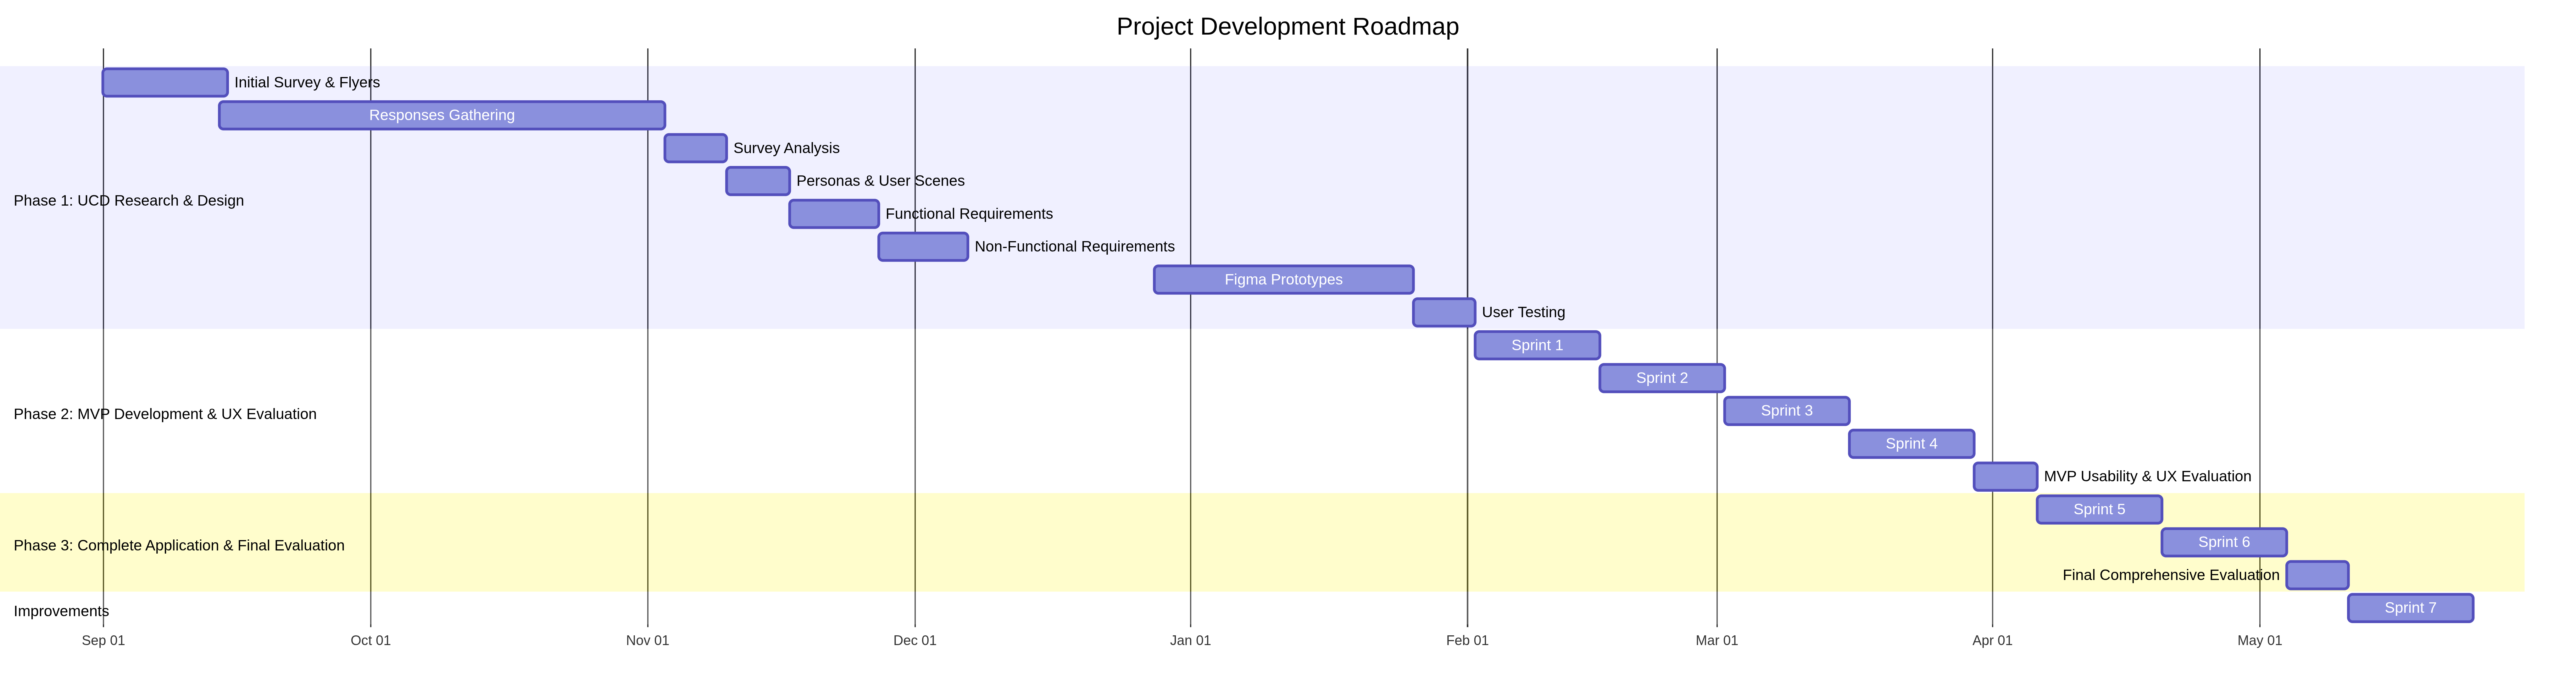
\includegraphics[width=1\textwidth]{figs/roadmap}
	\caption{Project Development Roadmap}
	\label{fig:roadmap}
\end{figure}


\subsection{Phase 1: Prototype and Feature Validation}

The first phase includes all four steps of UCD (\ref{subsec:ucd}) in order to research the problem, design a proposed solution and evaluate with the possible users. These are the steps that are carried out:

A survey is conducted to understand the basketball players who uses public courts, including their habits, challenges and desired improvements to their experience. With that, \textit{personas} are created representing different user needs and pain points. User scenarios are also developed for different contexts , describing how they use public courts, what problems they encounter and when and how a platform would support them. Through the \textit{personas} and scenarios, requirements are gathered to respond to their needs, documenting them as User Stories (see \ref{subsec:us-sprint-attd}) and added to the Jira project Backlog. The prototypes of User Stories are created in Figma to provide an interactive and testable design. Finally, users test the interactive prototype and provide feedback on the importance and relevance of the features. This feedback is used to update and prioritize the backlog for the next iterations. In this first phase, the tests that users will perform are Task-based usability testing using interactive Figma prototype, followed by a Feature Prioritization Survey assessing feature importance and relevance;

\subsection{Phase 2: MVP Development and UI/UX Evaluation}

In the second phase, instead of a prototype, a Minimum Viable Product (MVP) is developed, with the main features completed enough that can be usable in early stages and receive feedback. This phase starts applying both Scrum and ATDD methodologies (see \ref{subsec:us-sprint-attd} to implement the most critical user stories identified from the first phase's feedback. Each user story follows the ATDD approach, where acceptance criteria are defined, and tests are written to validate these criteria, the feature is developed and then validated ensuring all tests pass. User stories are organized into sprints according to the Scrum framework, enabling iterative and continuous progress, tracking on Jira. With a functional MVP, users evaluate the platform focusing on user experience (UX) and user interface (UI) aspects, through Task-Based Usability Testing to measure task performance, System Usability Scale (SUS) questionnaire combined with think-aloud protocol during task execution, and User Experience questionnaire, providing feedback to guide refinements in the final phase.

The \ref{fig:jiraRoadmap} repreesents the 5 Epics created that contain the User Stories, as well as the propose sprint planning, where from the Sprint 1 to 4 is the Phase 2 following a break to test, and sprint 5 and 6 represent the Phase 3 (the attribution of the User Stories to each sprint can be adjusted during its development, depending on the its progress ). The Epic prioritization follows a dependency-driven and value-driven approach. For this second phase it is more focuses on delivering the minimum feature set required to validate the core value proposition, enabling players to discover courts and organize games. 

\textit{User Profile and Settings (PLY-9)} is developed first in Sprint 1, as authentication and profile management are foundational requirements for all subsequent features. \textit{Court Availability (PLY-6)} is also initiated in Sprint 1, establishing the court discovery infrastructure that is fundamental to game creation. Sprints 2 implements \textit{Game Management (PLY-5)}, which represents the application's primary value, by creating, browsing, joining, and managing basketball games. This sequence ensures that users can complete the core user journey from registration through game participation, enabling meaningful usability evaluation.
In Sprint 3 and 4 is developed features from the different Epics that are not necessary for the main functionality but still adds important value for the application, including adding team and ranking system from the Epic \textit{Ranking and Team System (PLY-8)}. 

\begin{figure}[h]
	\centering
	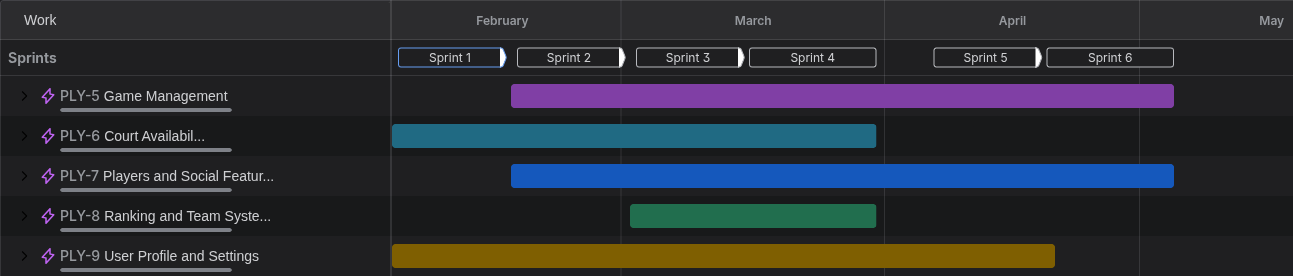
\includegraphics[width=1\textwidth]{figs/jiraSprintsRoadmap}
	\caption{Epics and Sprint planning in Jira}
	\label{fig:jiraRoadmap}
\end{figure}


\subsection{Phase 3: Complete Application and Overall Evaluation}

Following feedback from the second phase, in the final one it is developed the complete platform, continuing to apply Scrum and ATDD. Improvements from previous feedback are made and all remaining user stories are implemented, developing as well the tests first, ensuring consistent quality throughout. Users conduct a comprehensive evaluation of the complete platform, assessing overall functionality, usability, reliability and satisfaction with the final product, using SUS, task-based testing, and semi-structured interviews.

Continuing the analysis of the Figure \ref{fig:jiraRoadmap}, this phase stars in Sprint 5 and it adds value to the \textit{Game Management (PLY-5)} Epic and a chat function from the Epic \textit{Players and Social Features (PLY-7)}. It will also improve features and bugs detected in the testing in Phase 2, so the Sprints will likely change. 



\subsection{User Stories, Sprints and ATDD}\label{subsec:us-sprint-attd}

Requirements gathered during the second phase of UCD (Subsection \ref{subsec:ucd}) are documented as User Stories and integrated into Scrum's Sprint structure. User Stories employ non-technical language written from the user's perspective, clarifying not only what is being built, but also the rationale and value delivered\cite{userStoriesAtlassian}.  Normally, each User Story belongs to an Epic as milestones, representing a broader thematic organization, enabling progress tracking against major features.  Each story is assigned to a Sprint and marked as complete when users can successfully execute the outlined task, aligning with the project's emphasis on User-Centred Design throughout development. The User Story will be moved through different stages in a board, starting in the To-Do column, moved to the in progress, then testing where is checked if it passes the acceptance criteria initially defined, ending up in the done. Jira\footnote{https://www.atlassian.com/software/jira} serves as the project management tool, enabling systematic planning, task assignment, and progress tracking throughout the development phase. 

ATDD complements the Scrum framework by ensuring that acceptance tests are written for each User Story before implementation\cite{agileAllianceATDD}. This ensures requirements are precisely defined and verifiable, with tests serving as executable specifications of expected behaviour. The ATDD workflow follows three steps, starting by writing the acceptance tests to define expected behaviour, the feature is then implemented to satisfy these tests, and finally, functionality is validated to ensure all tests pass.This project employs rule-oriented acceptance criteria using a checklist format\cite{acceptanceCriteria}, which integrates naturally with the User Story structure in Jira. It could also be written in a scenario-oriented way, using a Given/When/Then template.

\section{Evaluation Strategy}
\label{sec:method-evaluation}

\subsection{System Usability Scale}
\label{subsec:method-sus}

\subsection{Task-Based Usability Testing}
\label{subsec:method-tasks}

\section{Project Roadmap}
\label{sec:method-roadmap}


\chapter{Methodology}



